% faros_main.tex -- Elsevier (elsarticle) manuscript.
% Compile from docs/: pdflatex, bibtex, pdflatex, pdflatex.
%
% Reading order for a reviewer:
%   the problem -> what existing solutions give -> what is missing
%   -> what we change -> why it should work -> what we measured.
%
% Every number comes from outputs/logs/burst_benchmark_full.json,
% outputs/logs/BENCHMARK_SUMMARY.json, outputs/logs/arrival_value.json and
% outputs/logs/burst_nonanticipative_probe.json. Sign tests and Holm values are
% recomputed from the per-day costs in burst_benchmark_full.json (10 contrasts).
% AUTHOR CHECK marks decisions only the authors can make. The reviewer backlog
% is in the comment block after \end{document}.
%%%%%%%%%%%%%%%%%%%%%%%%%%%%%%%%%%%%%%%%%%%%%%%%%%%%%%%%%%%%%%%%%%%%%%%%%%%%

\documentclass[5p,times,authoryear]{elsarticle}

\usepackage{graphicx}
\usepackage{amsmath,amssymb,amsthm}
\usepackage{booktabs}
\usepackage{array}
\usepackage{enumitem}
\usepackage[table]{xcolor}
\usepackage{tikz}
\usepackage{pgfplots}
\usepackage{algorithm}
\usepackage{algpseudocode}
\usepackage{placeins}
\usepackage{hyperref}

\usetikzlibrary{arrows.meta,positioning,fit,backgrounds,calc,shapes.geometric}
\pgfplotsset{compat=1.18}

\definecolor{farosgood}{RGB}{226,242,230}
\definecolor{cnear}{RGB}{150,150,150}
\definecolor{cmsa}{RGB}{214,120,40}
\definecolor{cwf}{RGB}{120,90,180}
\definecolor{chyb}{RGB}{31,119,180}
\definecolor{clazy}{RGB}{20,140,110}

\newtheorem{definition}{Definition}
\newtheorem{property}{Property}

\raggedbottom
\emergencystretch=1.5em
\setlength{\textfloatsep}{14pt plus 4pt minus 3pt}
\renewcommand{\topfraction}{0.9}
\renewcommand{\dbltopfraction}{0.9}
\renewcommand{\textfraction}{0.07}
\renewcommand{\floatpagefraction}{0.8}
\renewcommand{\dblfloatpagefraction}{0.8}
\setcounter{topnumber}{3}
\setcounter{dbltopnumber}{2}
\setcounter{totalnumber}{5}

% AUTHOR CHECK: target journal.
\journal{European Journal of Operational Research}

\begin{document}

\begin{frontmatter}

\title{Wait Before You Sample: Fork-Aware, Order-Bound Scenario Recourse for Dynamic Vehicle Routing with Clustered Requests}

% AUTHOR CHECK: final author list, affiliations, corresponding author.
% AUTHOR CHECK: department and author order for Zhiguang Cao.
\author[1]{Shreya Kumari}
\author[2]{Zhiguang Cao}
\address[1]{Technology Control Company, Riyadh, Saudi Arabia}
\address[2]{National University of Singapore, Singapore}

\begin{abstract}
A delivery vehicle often knows which customers it may have to visit during the day but not when each of them will place a request. When requests arrive in waves, one area after another, the vehicle repeatedly faces the same choice at the end of a wave: serve a nearby leftover customer, drive to a distant customer of the next wave, or wait for that wave to fill in. Existing methods handle this choice in one of two ways. Waiting rules decide when to move but route greedily. Scenario sampling simulates possible futures for every option, waiting included, and picks the option with the lowest average cost. We propose FAROS (Fork-Aware Recourse with Ordered Sampling), a simple combination: a waiting rule decides first, using only the known wave windows, and scenario sampling is used only when the rule says to move. We test this on a single-vehicle capacitated routing benchmark with a frozen set of 40 test days and measure the realized distance of each day's tour. Greedy nearest-customer dispatching drives 25.53 on average, scenario sampling 21.30, the waiting rule alone 20.89, and the two variants of our method 20.23 and 20.00. Both variants beat scenario sampling on 31 and 34 of the 40 days (Holm-adjusted sign test $p=0.003$ and $p<10^{-4}$), beat the waiting rule alone, and make 27--30\% fewer sampling calls. With five sampled futures our method is better than scenario sampling with twenty, which indicates that sampling noise in the wait-or-go comparison is what our method removes.
\end{abstract}

\begin{keyword}
Routing \sep Dynamic vehicle routing \sep Stochastic requests \sep Waiting strategies \sep Rollout \sep Scenario sampling
\end{keyword}

\end{frontmatter}

% AUTHOR CHECK: Elsevier requires 3--5 highlights (max 85 characters each)
% as a separate file. Suggested:
%  - Clustered request waves create a recurring wait-or-go choice
%  - A waiting rule decides first; scenario sampling is used only to route
%  - Tours are 5--6% shorter than with scenario sampling on all options
%  - The method needs about 30% fewer sampling calls and works with five samples
%  - Benchmark, frozen instances and paired tests are released

% =========================================================================
\section{Introduction}
\label{sec:intro}
% =========================================================================

\subsection{The problem}

Consider a vehicle that serves customers during a working day. The operator knows which customers may need a visit, where they are, and how much they need, from contracts, subscriptions, or history. It does not know \emph{when} each customer will place its request. A customer becomes visible only when its request arrives, and the vehicle can only serve visible customers. The goal is to serve everyone while driving as little as possible. This is a dynamic vehicle routing problem with stochastic request times \citep{psaraftis2016dynamic,pillac2013review,ritzinger2016survey}, and the version in which customer locations are known in advance has been studied by \citet{thomas2007waiting} and \citet{saintguillain2017ssvrptw}.

Requests are rarely spread evenly over the day. They often arrive in waves, one area after another: a business district opens, a shift ends, a campaign starts. Consecutive waves overlap in time. This creates a recurring choice that we call a \emph{fork} (Figure~\ref{fig:motivation}). The vehicle is finishing one wave and has a leftover customer nearby, while the first request of the next wave has appeared far away. It can serve the leftover, drive to the new wave now, or wait until more of the new wave is visible so that one long trip serves many customers. A vehicle that always takes the nearest visible customer makes the long trip for a single customer and may cross the area several times. Most of the avoidable distance is decided at these forks.

\subsection{What existing solutions give}

Table~\ref{tab:existing} summarizes the four families of methods that apply to this problem, what each one provides, and what it leaves open.

\begin{table*}[t]
\centering
\caption{Existing solutions for dynamic routing with uncertain request times, and what this paper takes from each.}
\label{tab:existing}
\footnotesize
\setlength{\tabcolsep}{4pt}
\renewcommand{\arraystretch}{1.15}
\begin{tabular}{@{}>{\raggedright\arraybackslash}p{0.17\textwidth}>{\raggedright\arraybackslash}p{0.25\textwidth}>{\raggedright\arraybackslash}p{0.25\textwidth}>{\raggedright\arraybackslash}p{0.27\textwidth}@{}}
\toprule
Family & What it gives & What it leaves open & Role in this paper \\
\midrule
Greedy dispatching and reoptimization \citep{gendreau1999parallel,larsen2002partially} & Fast, simple decisions based on visible requests & No anticipation: it never waits on purpose and makes the same long trip repeatedly & Nearest-customer dispatching is our baseline and is used at every non-fork decision \\
Scenario sampling and rollout \citep{bent2004scenario,vanhentenryck2006online,goodson2017rollout} & Anticipation: each option is simulated on sampled futures and the cheapest on average is chosen & Costly, and noisy with few samples; waiting is just one more option compared on noisy estimates & Our sampling stage; also our main comparison method \\
Waiting rules \citep{mitrovic2004waiting,branke2005waiting,thomas2007waiting} & Cheap, explicit decisions on \emph{when} to move & Routing after the wait stays greedy & Our first stage \\
Value approximation and learning \citep{ulmer2019adp,kool2019attention,baty2024combinatorial} & Fast decisions once a model is trained & Needs training data and design effort; behavior is hard to inspect & Secondary comparison only \\
\bottomrule
\end{tabular}
\end{table*}

The two families that address the fork directly are scenario sampling and waiting rules. Scenario sampling, in the tradition of \citet{bent2004scenario}, treats waiting as one option among several. At each fork it simulates the rest of the day for each option on a number of sampled futures and picks the option with the lowest average cost. Waiting rules, in the tradition of \citet{mitrovic2004waiting}, decide only when the vehicle should move and leave routing to a simple heuristic. When sampling methods include waiting, they let it compete with every routing option on the same sampled estimates \citep{bent2007waiting}.

\subsection{What is missing}

Waiting and routing are different kinds of decisions. Whether to wait depends mostly on how much of the current wave is still to come, and the operator already knows that from the wave's time window, without any sampling. Which customer to drive to depends on the detailed positions and timing of future requests, and sampling is well suited to estimate that. When both decisions are put into one comparison, the timing choice is made on noisy estimates, and sampling effort is spent on a question that known structure answers. We are not aware of work that settles the timing decision with a structural rule \emph{before} scenario sampling and measures the effect of doing so under the same simulator, base heuristic, and instances.

\subsection{What we do}

We call our method \textbf{FAROS}, for \emph{Fork-Aware Recourse with Ordered Sampling}. It is \emph{fork-aware} because it departs from greedy dispatching only at forks, and its sampling is \emph{ordered} because the timing decision is made before any simulation. FAROS keeps everything from scenario sampling except the order in which the two decisions are made (Figure~\ref{fig:method}):
\begin{enumerate}[label=\arabic*.,leftmargin=*,nosep,topsep=2pt]
\item At every decision that is not a fork, the vehicle serves the nearest visible customer.
\item At a fork, a \emph{waiting rule} is checked first. If the wave the vehicle is serving still has customers that have not appeared, the vehicle waits. This uses only the known wave windows and costs no sampling.
\item Otherwise scenario sampling decides. In the \emph{FAROS-Go} variant it chooses among the customers only. In the \emph{FAROS-All} variant it may still choose to wait.
\end{enumerate}
Both variants use exactly the same sampling procedure as the comparison method, so any difference in tour length comes from the order of the decisions.

\subsection{What we find}

On 40 paired test days, nearest dispatching drives 25.53 on average and scenario sampling 21.30. The waiting rule alone, with no sampling, reaches 20.89. FAROS-Go and FAROS-All reach 20.23 and 20.00, beat scenario sampling on 31 and 34 days, beat the waiting rule alone on 29 and 34 days, and make about 30\% fewer sampling calls. Scenario sampling improves markedly as the number of sampled futures grows, whereas our method barely changes. With five samples, our method is better than scenario sampling with twenty. This pattern indicates that our method removes sampling noise from the wait-or-go comparison.

\noindent\textbf{Contributions.}
\begin{enumerate}[leftmargin=*,nosep,topsep=2pt]
\item We identify the fork between consecutive request waves as the place where anticipation pays, and we restrict all non-greedy decisions to these forks (Section~\ref{sec:formulation}).
\item We propose to decide waiting first with a zero-sample rule and to use scenario sampling only for the remaining decision, in two variants (Section~\ref{sec:method}).
\item We provide a reproducible benchmark with frozen instances, fixed train/validation/test splits, and paired statistical tests on realized tour length (Section~\ref{sec:setup}).
\item We show that the change shortens tours, reduces sampling effort, and works with a small sampling budget, and we trace the gain to sampling noise (Section~\ref{sec:results}).
\end{enumerate}

% =========================================================================
\section{Related Work}
\label{sec:related}
% =========================================================================

\subsection{Dynamic and stochastic vehicle routing}

Dynamic vehicle routing problems change routes as information arrives during the day. \citet{psaraftis2016dynamic} review three decades of such problems and classify them by how information evolves. \citet{pillac2013review} and \citet{ritzinger2016survey} distinguish problems in which information is simply revealed over time from problems in which a probabilistic forecast of that information is available. The share of requests that is unknown at the start, the degree of dynamism, determines how much of a plan can be fixed in advance \citep{larsen2002partially}. \citet{bertsimas1991stochastic} analyze a stochastic and dynamic problem in the plane, and recent reviews focus on random requests during the day \citep{zhang2023dvrpreview} and on the use of forecasts \citep{soeffker2022prescriptive}. \citet{ulmer2020modeling} recommend modeling these problems as sequential decision processes with explicit decision times, states, and transitions; Section~\ref{sec:formulation} follows that advice.

Our problem belongs to the class with known potential customers and random request times. \citet{thomas2007waiting} studies waiting when customer locations are known and requests are probabilistic. \citet{saintguillain2017ssvrptw} study a variant with time windows in which both whether a customer appears and when it appears are random. In our setting every customer eventually appears, and request times are clustered in space and overlap in time, a structure that we exploit directly.

\subsection{Scenario sampling and rollout}

The simplest dynamic methods rerun a static solver whenever a request arrives \citep{gendreau1999parallel}. They react to new requests but do not anticipate future ones. Scenario-based methods add anticipation. \citet{bent2004scenario} keep a pool of sampled future scenarios, plan for each, and choose the decision that most plans agree on. \citet{vanhentenryck2006online} generalize this into a family of online stochastic methods. Its \emph{expectation} variant evaluates each candidate decision on every scenario and picks the best average, and our comparison method is of this type. Related approaches hedge over sample scenarios \citep{hvattum2006sample} or insert forecast requests into the plan \citep{ichoua2006exploiting,ghiani2009anticipatory}.

Rollout algorithms arrive at the same estimate from approximate dynamic programming \citep{powell2011adp}: a simple base heuristic is simulated forward from each candidate decision \citep{bertsekas1997rollout}. \citet{secomandi2001rollout} apply rollout to routing with stochastic demand, and \citet{goodson2013rollout,goodson2017rollout} give a general framework and show that rollout improves on its base heuristic. In these methods waiting, when available, is treated like any other decision.

\subsection{Waiting strategies}

A separate line of work asks when a vehicle should move. \citet{mitrovic2004waiting} compare drive-first, wait-first, and dynamic waiting for pickup and delivery with time windows and show that the waiting rule alone changes results substantially. \citet{branke2005waiting} study where and how long to wait so that late requests can still be served, and \citet{thomas2007waiting} derives waiting strategies from known customer locations. \citet{bent2007waiting} add waiting and relocation to scenario-based planning. There, waiting enters the sampled comparison as an extra option rather than being decided beforehand. Our method decides it beforehand.

\subsection{Value approximation and learning}

Approximate dynamic programming replaces sampling at decision time with a value function trained offline. \citet{ulmer2018budgeting} approximate the value of remaining time to decide which requests to accept, \citet{ulmer2019adp} combine offline value approximation with online rollouts, and \citet{voccia2019sameday} solve same-day delivery with sampled scenarios. Deep reinforcement learning for routing has mostly addressed the static problem with complete information \citep{nazari2018rl,kool2019attention}. For the dynamic problem, a recent competition was won by a learned model combined with a combinatorial solver \citep{baty2024combinatorial}. We include a simple learned dispatcher only to check whether the structural rule leaves gains that learning could capture (Sections~\ref{sec:uniform} and~\ref{sec:learned}).

% =========================================================================
\section{Problem Description}
\label{sec:formulation}
% =========================================================================

\subsection{A fork, step by step}
\label{sec:motivation}

\begin{figure*}[t]
\centering
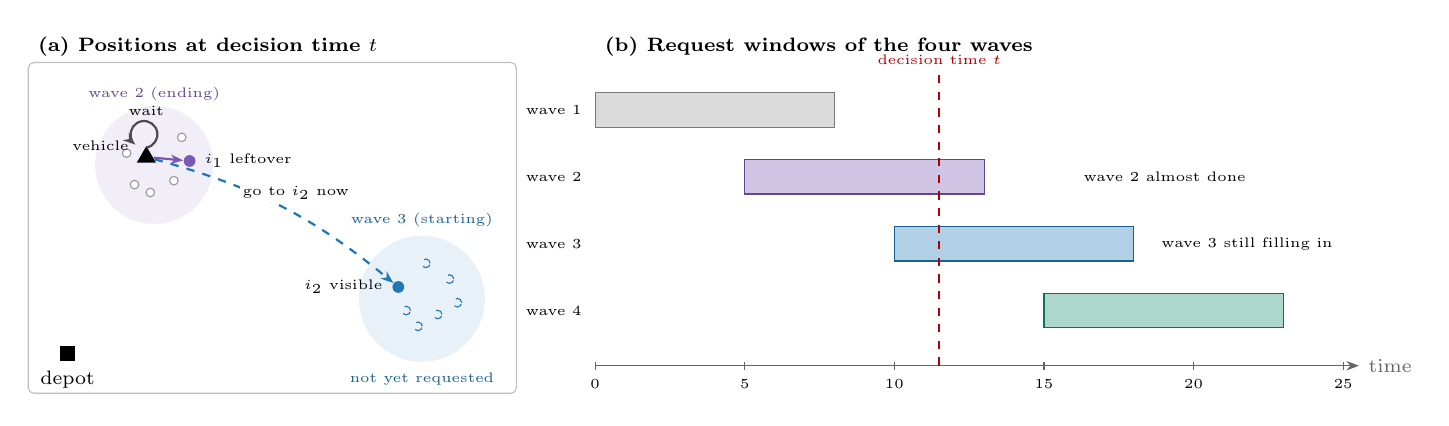
\begin{tikzpicture}[font=\scriptsize, >={Stealth[length=1.6mm]}]
\begin{scope}
  \draw[black!25, rounded corners=2pt] (0,0) rectangle (6.2,4.2);
  \node[anchor=north west, font=\scriptsize\bfseries] at (0,4.65) {(a) Positions at decision time $t$};
  \node[draw, fill=black, minimum size=5pt, inner sep=0pt] (dep) at (0.5,0.5) {};
  \node[anchor=north] at (dep.south) {depot};
  \fill[cwf!10] (1.6,2.9) circle (0.75);
  \node[font=\tiny, text=cwf!80!black] at (1.6,3.8) {wave 2 (ending)};
  \foreach \p in {(1.25,3.05),(1.55,2.55),(1.95,3.25),(1.85,2.7),(1.35,2.65)}
    \node[circle, draw=black!40, fill=white, inner sep=1.1pt] at \p {};
  \node[circle, fill=cwf, inner sep=1.5pt] (left) at (2.05,2.95) {};
  \node[anchor=west, font=\tiny] at (2.12,2.95) {$i_1$ leftover};
  \node[regular polygon, regular polygon sides=3, fill=black, inner sep=1.4pt] (veh) at (1.5,3.0) {};
  \node[anchor=east, font=\tiny] at (1.4,3.15) {vehicle};
  \fill[chyb!10] (5.0,1.2) circle (0.8);
  \node[font=\tiny, text=chyb!80!black] at (5.0,2.2) {wave 3 (starting)};
  \node[circle, fill=chyb, inner sep=1.5pt] (far) at (4.7,1.35) {};
  \node[anchor=east, font=\tiny] at (4.62,1.35) {$i_2$ visible};
  \foreach \p in {(5.2,1.0),(5.35,1.45),(4.95,0.85),(5.45,1.15),(5.05,1.65),(4.8,1.05)}
    \node[circle, draw=chyb, dashed, inner sep=1.1pt] at \p {};
  \node[font=\tiny, text=chyb!80!black, anchor=north] at (5.0,0.38) {not yet requested};
  \draw[->, cwf, thick] (veh) -- (left);
  \draw[->, chyb, thick, dashed] (veh) to[bend left=12] (far);
  \node[font=\tiny, fill=white, inner sep=1pt] at (3.4,2.55) {go to $i_2$ now};
  \draw[->, black!70, thick] (veh) ++(0,0.12) arc[start angle=-80, end angle=230, radius=0.17];
  \node[font=\tiny, anchor=south] at (1.5,3.4) {wait};
\end{scope}
\begin{scope}[xshift=7.2cm]
  \node[anchor=north west, font=\scriptsize\bfseries] at (0,4.65) {(b) Request windows of the four waves};
  \def\sx{0.38}
  \draw[->, black!60] (0,0.35) -- (25*\sx+0.2,0.35) node[anchor=west] {time};
  \foreach \x in {0,5,10,15,20,25} {
    \draw[black!60] (\x*\sx,0.3) -- (\x*\sx,0.4);
    \node[anchor=north, font=\tiny] at (\x*\sx,0.3) {\x};
  }
  \foreach \k/\c/\y in {1/cnear/3.6,2/cwf/2.75,3/chyb/1.9,4/clazy/1.05} {
    \pgfmathsetmacro{\s}{(\k-1)*5}
    \fill[\c!35] (\s*\sx,\y-0.22) rectangle ({(\s+8)*\sx},\y+0.22);
    \draw[\c!80!black] (\s*\sx,\y-0.22) rectangle ({(\s+8)*\sx},\y+0.22);
    \node[anchor=east, font=\tiny] at (-0.05,\y) {wave \k};
  }
  \draw[red!70!black, thick, dashed] (11.5*\sx,0.35) -- (11.5*\sx,4.05);
  \node[anchor=south, font=\tiny, text=red!70!black] at (11.5*\sx,4.05) {decision time $t$};
  \node[font=\tiny, anchor=west] at (16*\sx,2.75) {wave 2 almost done};
  \node[font=\tiny, anchor=west] at (18.6*\sx,1.9) {wave 3 still filling in};
\end{scope}
\end{tikzpicture}
\caption{A fork, drawn for illustration with the benchmark settings of Section~\ref{sec:benchmark}. (a) The vehicle is finishing wave 2. A leftover customer $i_1$ is close; the first visible customer $i_2$ of wave 3 is far away; most of wave 3 has not requested yet. (b) Each wave places its requests at random within a window of 8 time units, and consecutive windows overlap by 3. At time $t$ wave 3 has started but is far from complete. Driving to $i_2$ now serves one customer per long trip; waiting lets one trip serve most of the wave.}
\label{fig:motivation}
\end{figure*}

Figure~\ref{fig:motivation} shows the decision this paper is about. The vehicle is finishing wave 2 and has one leftover customer $i_1$ nearby. Wave 3 has started far away, and only one of its customers, $i_2$, is visible. A nearest-customer dispatcher serves $i_1$, then finds $i_2$ to be the only visible customer and drives to it. When it arrives, most of wave 3 has still not requested. It then waits there or drives back toward other leftovers, and in the worst case it crosses the area several times for the same wave. Had it waited briefly, the long trip to wave 3 would have served many customers at once.

Two observations shape our method. Whether waiting is worthwhile depends mainly on how much of the newest wave is still missing, and that follows from the known wave window. Which customer to drive to next depends on exactly where and when the missing customers will appear, and that is what sampling estimates.

\subsection{Formal description}

\paragraph{Instance}
A depot $0$ and customers $\mathcal{N}=\{1,\dots,n\}$ lie in the unit square. Customer $i$ has a location, a demand $d_i$, and belongs to a wave with request window $[w_i,w_i+W]$. One vehicle with capacity $Q$ drives at unit speed, so driving time equals Euclidean distance $c_{ij}$. Customer $i$ requests at a random time $r_i$, uniform in its window, and becomes visible at that time.

\paragraph{What the dispatcher knows}
The dispatcher knows all customers, their locations and demands, and the wave windows in advance. It does not know the request times $r=(r_i)_{i\in\mathcal{N}}$. At time $t$ it sees which customers have requested, $\mathcal{R}_t=\{i:r_i\le t\}$.

\paragraph{Decisions}
Decisions are made whenever the vehicle stands still: after serving a customer, after a depot visit, or after a wait \citep{ulmer2020modeling}. Requests that arrive while the vehicle drives are seen at the next stop. The state is
\begin{equation}
s=(t,\ \ell,\ q,\ \mathcal{V},\ \mathcal{R}_t),
\label{eq:state}
\end{equation}
namely time, vehicle location, remaining capacity, served customers, and visible customers. A customer is \emph{feasible} if it is visible, unserved, and its demand fits: $F(s)=\{i\in\mathcal{R}_t\setminus\mathcal{V}: d_i\le q\}$. The vehicle can go to a feasible customer, return to the depot to reload, or wait until the next request appears, which costs no distance.

\paragraph{Objective}
A policy $\pi$ chooses an action in every state. Its cost on a day with request times $r$ is the total distance driven until all customers are served and the vehicle is back at the depot, $C(\pi;r)$. We seek
\begin{equation}
\min_{\pi}\ \mathbb{E}_{r}\bigl[C(\pi;r)\bigr].
\label{eq:objective}
\end{equation}
Waiting costs no distance but uses time. Its value shows only in the tour that follows, so we always measure complete tours and never score a single decision on its own.

\subsection{Nearest dispatching and forks}

The \emph{nearest dispatcher} $\pi^{\mathrm{N}}$ goes to the nearest feasible customer. If no customer is feasible and visible customers remain, it returns to the depot. Otherwise it waits for the next request.

\begin{definition}[Fork]
Let $D(s)$ be up to $K$ feasible customers chosen in order of distance from the vehicle, keeping a customer only if it is at least $\delta$ away from every customer already kept. State $s$ is a \emph{fork} if $t<H$ and $D(s)$ contains at least two customers. The options at a fork are
\begin{equation}
\mathcal{A}(s)=\{\text{go to } i: i\in D(s)\}\ \cup\ \{\text{wait, if some customer has not requested yet}\}.
\label{eq:forkactions}
\end{equation}
\end{definition}

We use $K=4$, $\delta=0.25$, and $H=40$. Separated candidates are, in practice, customers in different waves or far apart within one wave. Every policy in this paper behaves like the nearest dispatcher outside forks and differs only in how it chooses from $\mathcal{A}(s)$ at forks.

\subsection{Scenario sampling}

Scenario sampling estimates the cost of an option $a$ by simulation. It draws $M$ possible futures. In each future, every customer that has not requested yet receives a request time drawn uniformly from the part of its window that lies after $t$. For each future, the method applies $a$, completes the day with the nearest dispatcher, and records the distance. The estimate is the average,
\begin{equation}
\widehat{Q}_M(s,a)=\frac{1}{M}\sum_{m=1}^{M}C^{\mathrm{N}}(s,a;\omega_m).
\label{eq:qhat}
\end{equation}
This is a one-step rollout of the nearest dispatcher \citep{bertsekas1997rollout} and the expectation variant of scenario-based planning \citep{vanhentenryck2006online}. The comparison method, which we call \emph{sampling}, picks $\arg\min_{a\in\mathcal{A}(s)}\widehat{Q}_M(s,a)$ at every fork, with waiting as one of the options.

\paragraph{Hypothesis}
Each estimate in Eq.~\eqref{eq:qhat} has sampling error of order $1/\sqrt{M}$. Sampling therefore decides between waiting and going by comparing noisy numbers. If a rule based on the known wave windows makes the timing decision instead, and sampling only chooses among the remaining options, tours should become shorter. The advantage should also be largest when $M$ is small and shrink as $M$ grows. Section~\ref{sec:ablation-m} tests both predictions.

% =========================================================================
\section{FAROS: Wait First, Then Sample}
\label{sec:method}
% =========================================================================

\subsection{Overview}

Figure~\ref{fig:method} compares the decision flow of sampling with that of our method. Outside forks nothing changes. At a fork, sampling sends every option, waiting included, to the simulation. Our method first applies a waiting rule and calls the simulation only if the rule does not wait.

\begin{figure*}[t]
\centering
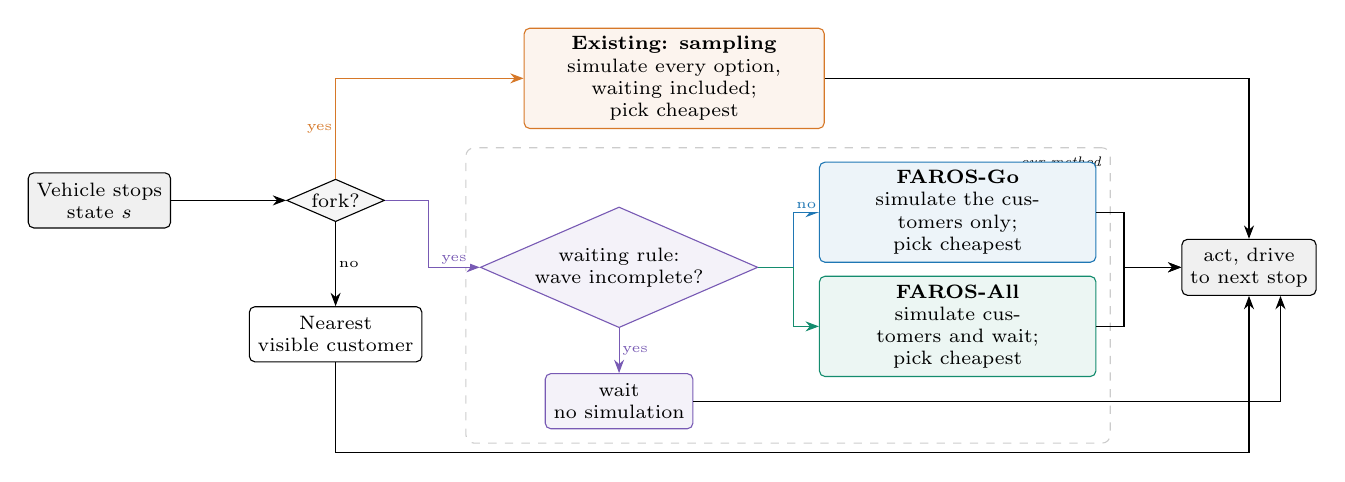
\begin{tikzpicture}[
  font=\scriptsize, >={Stealth[length=1.7mm]},
  box/.style={draw, rounded corners=2pt, align=center, inner sep=3pt, fill=white, minimum height=7mm},
  dec/.style={draw, diamond, aspect=2.3, align=center, inner sep=1pt, fill=black!4},
  lab/.style={font=\tiny, fill=white, inner sep=1pt}
]
\node[box, fill=black!6] (epoch) at (0,0) {Vehicle stops\\ state $s$};
\node[dec] (fork) at (3.0,0) {fork?};
\node[box] (back) at (3.0,-1.7) {Nearest\\ visible customer};
\draw[->] (epoch) -- (fork);
\draw[->] (fork) -- node[lab, right] {no} (back);

\node[box, draw=cmsa, fill=cmsa!8, text width=36mm] (full) at (7.3,1.55)
  {\textbf{Existing: sampling}\\ simulate every option,\\ waiting included; pick cheapest};
\node[dec, draw=cwf, fill=cwf!8] (screen) at (6.6,-0.85) {waiting rule:\\ wave incomplete?};
\node[box, draw=cwf, fill=cwf!8] (wait) at (6.6,-2.55) {wait\\ no simulation};
\node[box, draw=chyb, fill=chyb!8, text width=33mm] (hyb) at (10.9,-0.15)
  {\textbf{FAROS-Go}\\ simulate the customers only;\\ pick cheapest};
\node[box, draw=clazy, fill=clazy!8, text width=33mm] (FAROS-All) at (10.9,-1.6)
  {\textbf{FAROS-All}\\ simulate customers and wait;\\ pick cheapest};

\draw[->, cmsa] (fork.north) |- node[lab, pos=0.25, left] {yes} (full.west);
\draw[->, cwf] (fork.east) -- ++(0.55,0) |- node[lab, pos=0.75, above] {yes} (screen.west);
\draw[->, cwf] (screen) -- node[lab, right] {yes} (wait);
\draw[->, chyb] (screen.east) -- ++(0.45,0) |- node[lab, pos=0.75, above] {no} (hyb.west);
\draw[->, clazy] (screen.east) -- ++(0.45,0) |- (FAROS-All.west);

\node[box, fill=black!6] (act) at (14.6,-0.85) {act, drive\\ to next stop};
\draw[->] (full.east) -| (act.north);
\draw[->] (hyb.east) -- ++(0.35,0) |- (act.west);
\draw[->] (FAROS-All.east) -- ++(0.35,0) |- (act.west);
\draw[->] (wait.east) -| ([xshift=4mm]act.south);
\draw[->] (back.south) -- ++(0,-1.15) -| (act.south);

\begin{scope}[on background layer]
\node[draw=black!20, dashed, rounded corners=3pt, fit=(screen)(wait)(hyb)(FAROS-All), inner sep=5pt,
  label={[font=\tiny\itshape, anchor=north east]north east:our method}] {};
\end{scope}
\end{tikzpicture}
\caption{Decision flow of the existing sampling method (top) and of our method (dashed box). Both use the nearest customer outside forks and the same simulation, Eq.~\eqref{eq:qhat}. Our method first checks a waiting rule that needs no simulation and simulates only when the rule says to move. FAROS-Go then chooses among customers; FAROS-All may still choose to wait.}
\label{fig:method}
\end{figure*}

\subsection{Step 1: the waiting rule}

The rule asks one question: is the wave the vehicle is currently serving still producing requests? Let $a^\star$ be the customer that requested most recently among those not yet served, and let $u$ be the number of customers of the same wave that have not requested yet. If $u=0$ the rule does not wait. If $u\ge1$, the expected time until the first of them requests is at most half the remaining window, and the rule waits if that time is at most $\Delta=4$. In this benchmark the window is 8 long, so this condition always holds when $u\ge1$, and the rule simplifies to \emph{wait while the current wave is incomplete}. The rule uses only the known windows, never the actual request times.

On its own, with the nearest dispatcher after it, the rule is a \emph{wait-first} strategy in the sense of \citet{mitrovic2004waiting}, and we evaluate it as a separate policy.

\subsection{Step 2: sampling for the remaining decision}

If the rule does not wait, Eq.~\eqref{eq:qhat} decides. The two variants differ in one detail:
\begin{itemize}[leftmargin=*,nosep,topsep=2pt]
\item \textbf{FAROS-Go} simulates only the go-options. If fewer than two exist, it goes to the nearest customer without sampling.
\item \textbf{FAROS-All} simulates all options in $\mathcal{A}(s)$, waiting included. It accepts the rule's decision to wait but can still wait when the rule would not.
\end{itemize}
Algorithm~\ref{alg:method} gives the full procedure.

\begin{algorithm}[t]
\caption{Wait first, then sample (one decision)}
\label{alg:method}
\begin{algorithmic}[1]
\Require state $s$; number of futures $M$; variant \textsc{Go} or \textsc{All}
\If{$s$ is not a fork}
  \State \Return nearest feasible customer (or depot / wait as in $\pi^{\mathrm{N}}$)
\EndIf
\If{the current wave still has customers that have not requested}
  \State \Return wait \Comment{no simulation}
\EndIf
\If{variant is \textsc{Go}}
  \State $\mathcal{A}'\gets$ go-options in $\mathcal{A}(s)$
  \If{$|\mathcal{A}'|\le 1$} \Return nearest feasible customer \EndIf
\Else
  \State $\mathcal{A}'\gets\mathcal{A}(s)$ \Comment{waiting kept as an option}
\EndIf
\State draw $M$ futures; compute $\widehat{Q}_M(s,a)$ for every $a\in\mathcal{A}'$ \Comment{Eq.~\eqref{eq:qhat}}
\State \Return $\arg\min_{a\in\mathcal{A}'}\widehat{Q}_M(s,a)$
\end{algorithmic}
\end{algorithm}

\subsection{Why this should work}

\emph{Less noise in the timing decision.} Under sampling, a single unlucky future can make waiting look worse than going, or the reverse. The rule takes this decision without noise, so sampling only has to rank customers.

\emph{No effort on known structure.} That the current wave is incomplete is known from its window. Estimating the value of waiting by simulation at every fork spends computation to approximate a fact that is already available.

\emph{Fewer simulations.} Every fork at which the rule waits needs no simulation. FAROS-Go also drops the waiting option from each remaining simulation, so each call simulates at most $K M$ futures instead of $(K+1)M$.

\subsection{What is held fixed}

\begin{property}[Same behavior outside forks]\label{prop:backbone}
All policies act like the nearest dispatcher at every non-fork decision.
\end{property}

\begin{property}[Same simulation]\label{prop:estimator}
Sampling, FAROS-Go, and FAROS-All use the same estimate, Eq.~\eqref{eq:qhat}: the same base heuristic, the same distribution of futures, and the same $M$. They differ only in whether the waiting rule comes first and in which options are simulated.
\end{property}

\begin{property}[No look-ahead]\label{prop:nonanticipative}
No policy uses actual future request times. They are used only by the simulator that plays out the day.
\end{property}

Properties~\ref{prop:backbone} and~\ref{prop:estimator} make the comparison controlled: on the same day, a difference between sampling and our method can only come from the order of the decisions.

\begin{table}[t]
\centering
\caption{The five compared policies. All behave like the nearest dispatcher outside forks.}
\label{tab:policies}
\footnotesize
\setlength{\tabcolsep}{3pt}
\begin{tabular}{@{}llll@{}}
\toprule
Policy & At a fork, timing & At a fork, routing & Simulation \\
\midrule
Nearest & nearest dispatcher & nearest & none \\
Sampling & simulated & simulated & every fork \\
Wait rule & rule & nearest & none \\
FAROS-Go & rule & simulated, customers only & when rule moves \\
FAROS-All & rule, then simulated & simulated & when rule moves \\
\bottomrule
\end{tabular}
\end{table}

\paragraph{Computational effort}
Completing a day with the nearest dispatcher takes at most $O(n^2)$ operations. One sampling call therefore costs $O(|\mathcal{A}'|\,M\,n^2)$, and the waiting rule costs $O(n)$. The total effort is driven by the number of forks at which the rule does not wait, which Section~\ref{sec:compute} reports. The futures of one call are simulated as one vectorized batch.

% =========================================================================
\section{Experimental Setup}
\label{sec:setup}
% =========================================================================

\subsection{Questions}

\begin{enumerate}[label=(Q\arabic*),leftmargin=*,nosep,topsep=2pt]
\item Do non-greedy decisions at forks shorten tours compared with nearest dispatching?
\item Does our method shorten tours compared with sampling on the same days?
\item Does the sampling step add anything once the waiting rule is in place?
\item Does the advantage depend on the number of futures $M$, as the hypothesis predicts?
\item How much simulation does each policy need?
\item Would a learned dispatcher capture the same gains?
\end{enumerate}

\subsection{Benchmark}
\label{sec:benchmark}

Table~\ref{tab:params} lists the instance generator. Each day has 200 customers in four tight clusters whose centers are at least 0.45 apart. Cluster $k$ places its requests uniformly in the window $[5(k-1),\,5(k-1)+8]$, so consecutive waves overlap by 3 time units. Demands are integers from 1 to 9 and the capacity is 80, so the vehicle reloads at the depot several times a day.

\begin{table}[t]
\centering
\caption{Benchmark and policy parameters.}
\label{tab:params}
\footnotesize
\setlength{\tabcolsep}{4pt}
\begin{tabular}{@{}lr@{}}
\toprule
Parameter & Value \\
\midrule
Customers / waves & 200 / 4 \\
Capacity / demand per customer & 80 / 1--9 \\
Cluster spread (std.) / min.\ center distance & 0.015 / 0.45 \\
Wave start spacing / window length $W$ & 5 / 8 \\
Fork: candidates $K$ / separation $\delta$ / horizon $H$ & 4 / 0.25 / 40 \\
Waiting rule: same-wave tolerance / $\Delta$ & 0.5 / 4 \\
Futures per sampling call $M$ & 20 (also 5, 10) \\
Seeds / days per seed & 1234--1243 / 20 \\
Training / validation / test days & 0--11 / 12--15 / 16--19 \\
\bottomrule
\end{tabular}
\end{table}

Figure~\ref{fig:protocol} shows the protocol. For each of ten seeds, twenty days are generated once and stored, so every policy faces exactly the same days with exactly the same request times. Days 0--15 are used only to train and select the learned dispatcher; all reported results are on days 16--19. This gives 40 test days, and every comparison is paired by day.

\begin{figure*}[t]
\centering
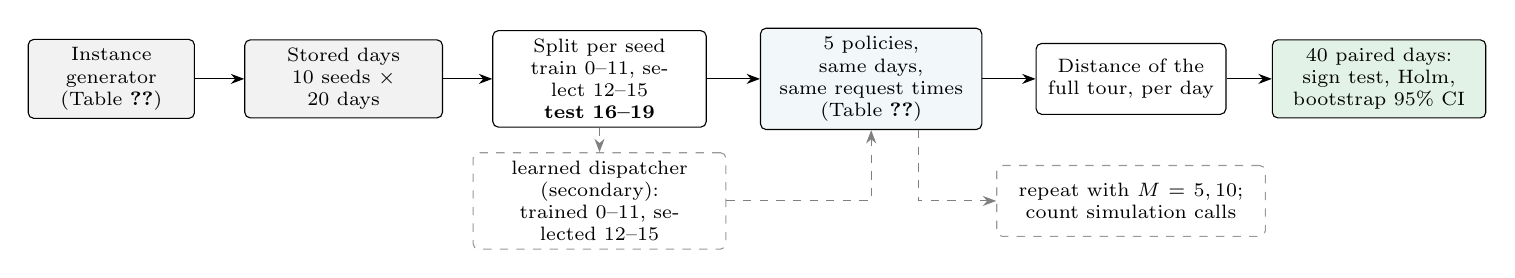
\begin{tikzpicture}[
  font=\scriptsize, >={Stealth[length=1.7mm]},
  box/.style={draw, rounded corners=2pt, align=center, inner sep=3pt, fill=white, minimum height=9mm, text width=#1},
  box/.default=22mm
]
\node[box=19mm, fill=black!5] (gen) at (0,0) {Instance generator\\ (Table~\ref{tab:params})};
\node[box=23mm, fill=black!5] (bank) at (2.95,0) {Stored days\\ 10 seeds $\times$ 20 days};
\node[box=25mm] (split) at (6.2,0) {Split per seed\\ train 0--11, select 12--15\\ \textbf{test 16--19}};
\node[box=26mm, fill=chyb!6] (pol) at (9.65,0) {5 policies, same days,\\ same request times\\ (Table~\ref{tab:policies})};
\node[box=22mm] (cost) at (12.95,0) {Distance of the\\ full tour, per day};
\node[box=25mm, fill=farosgood] (stat) at (16.1,0) {40 paired days:\\ sign test, Holm,\\ bootstrap 95\% CI};
\draw[->] (gen) -- (bank);
\draw[->] (bank) -- (split);
\draw[->] (split) -- (pol);
\draw[->] (pol) -- (cost);
\draw[->] (cost) -- (stat);
\node[box=30mm, draw=black!40, dashed] (learn) at (6.2,-1.55) {learned dispatcher (secondary):\\ trained 0--11, selected 12--15};
\draw[->, black!50, dashed] (split) -- (learn);
\draw[->, black!50, dashed] (learn.east) -| (pol.south);
\node[box=32mm, draw=black!40, dashed] (abl) at (12.95,-1.55) {repeat with $M=5,10$;\\ count simulation calls};
\draw[->, black!50, dashed] (pol.south) ++(0.6,0) |- (abl.west);
\end{tikzpicture}
\caption{Evaluation protocol. Days are generated once and stored, so all policies are compared on identical days. The learned dispatcher never sees the test days.}
\label{fig:protocol}
\end{figure*}

\subsection{Compared policies}

We compare the five policies of Table~\ref{tab:policies} with $M=20$. The sampling streams are seeded from the instance seed, identically for every sampling policy. As secondary results we report a learned dispatcher (Section~\ref{sec:learned}) and a check on days without waves (Section~\ref{sec:uniform}).

\subsection{Measurements and tests}

The main measurement is the distance of each complete tour, averaged over the 40 test days. We also report the standard deviation of the ten per-seed averages.

Each comparison between two policies is paired by day. We report the mean saving $\bar\Delta$ (distance of the reference minus distance of the policy), a 95\% bootstrap interval (2,000 resamples), and the number of days on which the policy is better, worse, or tied. The exact two-sided sign test checks whether the policy is better on more days than chance would explain, without assuming anything about the size of the differences. We correct the ten contrasts of Table~\ref{tab:paired} with the procedure of \citet{holm1979simple} and call a result supported if its adjusted $p$-value is below $0.05$.

\subsection{Reproducibility}

One script generates or loads the stored days, runs all policies and the $M$ variations, and writes every per-day result to a single log, from which all tables are computed.
% AUTHOR CHECK: repository URL or archive DOI, commit hash, Python/NumPy
% versions, hardware.

% =========================================================================
\section{Results}
\label{sec:results}
% =========================================================================

\subsection{Tour length}
\label{sec:main-results}

Table~\ref{tab:main} and Figure~\ref{fig:main-bars} report the average tour length (Q1, Q2). Every non-greedy policy shortens the tour by 4.2 to 5.5 units, 17\% to 22\% of the nearest dispatcher's distance. Of these, sampling is the weakest. The waiting rule alone, with no simulation, is already slightly better than sampling, and the two variants of our method are best.

\begin{table}[t]
\centering
\footnotesize
\caption{Average tour length over 40 test days (10 seeds $\times$ 4 days), $M=20$. Lower is better. $\bar\Delta$ is the average saving per day relative to the named policy.}
\label{tab:main}
\setlength{\tabcolsep}{3pt}
\begin{tabular}{@{}lrrrr@{}}
\toprule
Policy & Avg.\ tour & SD (seeds) & $\bar\Delta$ vs.\ nearest & $\bar\Delta$ vs.\ sampling \\
\midrule
Nearest & 25.53 & 1.34 & --- & --- \\
Sampling & 21.30 & 1.93 & 4.23 & --- \\
Wait rule & 20.89 & 1.91 & 4.65 & 0.42 \\
FAROS-Go & 20.23 & 1.67 & 5.30 & 1.07 \\
FAROS-All & \cellcolor{farosgood}\textbf{20.00} & 1.92 & \cellcolor{farosgood}\textbf{5.53} & \cellcolor{farosgood}\textbf{1.30} \\
\bottomrule
\end{tabular}
\end{table}

```latex
\begin{figure}[t]
\centering
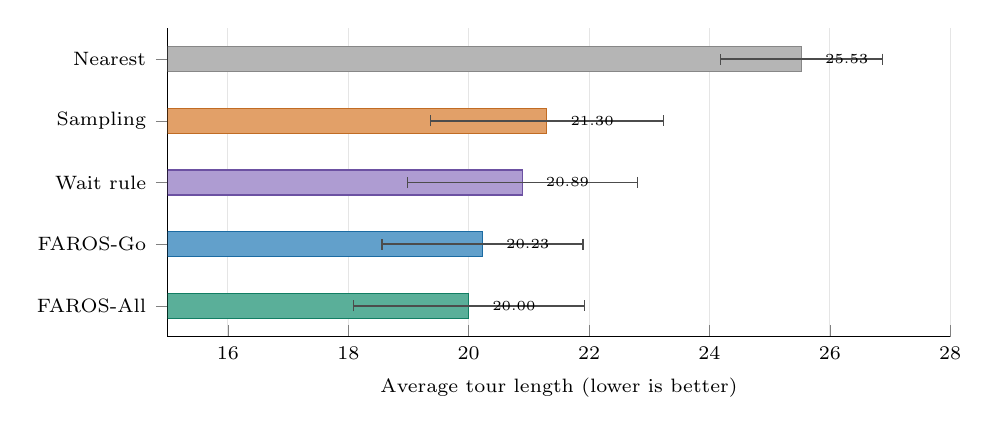
\begin{tikzpicture}
\begin{axis}[
    width=0.95\columnwidth,
    height=5.5cm,
    xbar,
    bar width=9pt,
    xmin=15,
    xmax=28,
    ymin=0.5,
    ymax=5.5,
    y dir=reverse,
    ytick={1,2,3,4,5},
    yticklabels={Nearest, Sampling, Wait rule, FAROS-Go, FAROS-All},
    enlarge y limits=false,
    xlabel={Average tour length (lower is better)},
    xmajorgrids,
    grid style={gray!20},
    axis lines*=left,
    tick label style={font=\scriptsize},
    label style={font=\scriptsize},
    nodes near coords,
    nodes near coords style={font=\tiny,anchor=west,xshift=5pt},
    point meta=explicit symbolic,
    error bars/x dir=both,
    error bars/x explicit,
    error bars/error bar style={black!70,line width=0.7pt}
]
\addplot[fill=cnear!70,draw=cnear!90!black,bar shift=0pt]
coordinates {(25.53,1) +- (1.34,0) [25.53]};

\addplot[fill=cmsa!70,draw=cmsa!90!black,bar shift=0pt]
coordinates {(21.30,2) +- (1.93,0) [21.30]};

\addplot[fill=cwf!60,draw=cwf!90!black,bar shift=0pt]
coordinates {(20.89,3) +- (1.91,0) [20.89]};

\addplot[fill=chyb!70,draw=chyb!90!black,bar shift=0pt]
coordinates {(20.23,4) +- (1.67,0) [20.23]};

\addplot[fill=clazy!70,draw=clazy!90!black,bar shift=0pt]
coordinates {(20.00,5) +- (1.92,0) [20.00]};
\end{axis}
\end{tikzpicture}
\caption{Average tour length on the 40 test days. Error bars indicate the standard deviation of the ten per-seed averages. The axis starts at 15.}
\label{fig:main-bars}
\end{figure}
```


\subsection{Day-by-day comparison}

Table~\ref{tab:paired} and Figure~\ref{fig:paired} compare the policies day by day.

\emph{Against nearest dispatching (Q1).} Every other policy is better on all 40 days.

\emph{Against sampling (Q2).} FAROS-Go is better on 31 days and FAROS-All on 34, and both intervals lie clearly above zero (adjusted $p=0.003$ and $p=5\times10^{-5}$). The waiting rule alone is better on 26 days, but its interval includes zero and the adjusted $p$-value is $0.16$, so its advantage over sampling is not established.

\emph{Against the waiting rule alone (Q3).} FAROS-Go is better on 29 days and FAROS-All on 34 (adjusted $p=0.019$ and $p=5\times10^{-5}$). The sampling step therefore adds value once the rule has decided when to wait; the method is more than a waiting rule.

\emph{FAROS-Go against FAROS-All.} FAROS-All is better on 20 days, worse on 16, and tied on 4 ($p=0.62$). The data do not separate the two variants.

\begin{table}[t]
\centering
\footnotesize
\caption{Day-by-day comparisons on 40 test days. $\bar\Delta>0$: the first policy drives less. W/L/T: days better, worse, tied. Exact two-sided sign test, Holm-corrected over the ten contrasts.}
\label{tab:paired}
\setlength{\tabcolsep}{2.5pt}
\begin{tabular}{@{}llrcrr@{}}
\toprule
Policy & Reference & $\bar\Delta$ & 95\% CI & W/L/T & $p_{\mathrm{Holm}}$ \\
\midrule
Sampling & Nearest & 4.23 & [3.61, 4.84] & 40/0/0 & $<10^{-10}$ \\
Wait rule & Nearest & 4.65 & [4.11, 5.22] & 40/0/0 & $<10^{-10}$ \\
FAROS-Go & Nearest & 5.30 & [4.76, 5.85] & 40/0/0 & $<10^{-10}$ \\
FAROS-All & Nearest & 5.53 & [4.99, 6.09] & 40/0/0 & $<10^{-10}$ \\
\midrule
Wait rule & Sampling & 0.42 & [$-$0.05, 0.88] & 26/14/0 & 0.161 \\
FAROS-Go & Sampling & 1.07 & [0.72, 1.41] & 31/9/0 & 0.003 \\
FAROS-All & Sampling & 1.30 & [0.96, 1.65] & 34/6/0 & $5\times10^{-5}$ \\
\midrule
FAROS-Go & Wait rule & 0.66 & --- & 29/11/0 & 0.019 \\
FAROS-All & Wait rule & 0.88 & --- & 34/6/0 & $5\times10^{-5}$ \\
\midrule
FAROS-All & FAROS-Go & 0.23 & --- & 20/16/4 & 0.618 \\
\bottomrule
\end{tabular}
\end{table}
% AUTHOR CHECK: bootstrap intervals for the last three rows are not in the log;
% add them by running paired_analysis() on those pairs.

\begin{figure}[t]
\centering
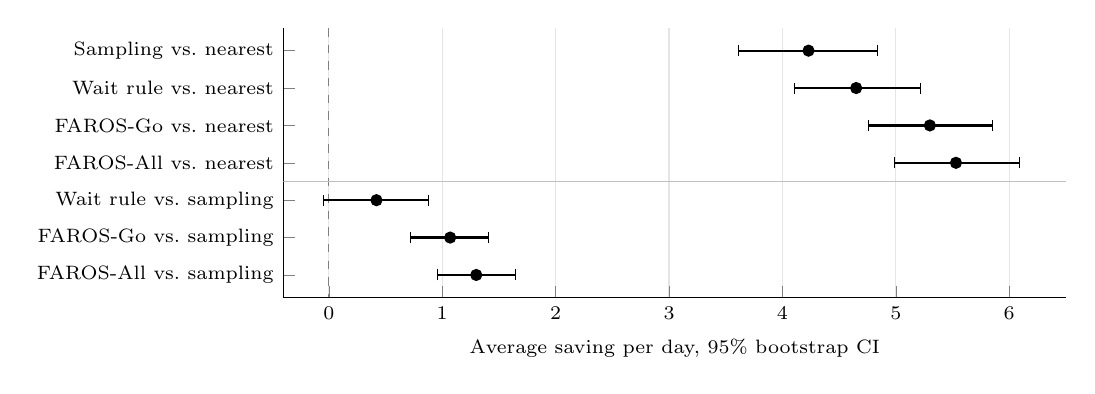
\begin{tikzpicture}
\begin{axis}[
  width=0.95\columnwidth, height=5.0cm,
  xmin=-0.4, xmax=6.5,
  ymin=0.4, ymax=7.6,
  y dir=reverse,
  ytick={1,2,3,4,5,6,7},
  yticklabels={Sampling vs.\ nearest, Wait rule vs.\ nearest, FAROS-Go vs.\ nearest, FAROS-All vs.\ nearest, Wait rule vs.\ sampling, FAROS-Go vs.\ sampling, FAROS-All vs.\ sampling},
  xlabel={Average saving per day, 95\% bootstrap CI},
  xmajorgrids, grid style={gray!20},
  axis lines*=left,
  tick label style={font=\scriptsize}, label style={font=\scriptsize}
]
\addplot[gray, dashed] coordinates {(0,0.4) (0,7.6)};
\draw[black!25] (axis cs:-0.4,4.5) -- (axis cs:6.5,4.5);
\addplot[only marks, mark=*, mark size=2pt, black,
  error bars/.cd, x dir=both, x explicit, error bar style={line width=0.8pt}]
coordinates {
  (4.23,1) += (0.61,0) -= (0.62,0)
  (4.65,2) += (0.57,0) -= (0.54,0)
  (5.30,3) += (0.55,0) -= (0.54,0)
  (5.53,4) += (0.56,0) -= (0.54,0)
  (0.42,5) += (0.46,0) -= (0.47,0)
  (1.07,6) += (0.34,0) -= (0.35,0)
  (1.30,7) += (0.35,0) -= (0.34,0)
};
\end{axis}
\end{tikzpicture}
\caption{Average saving per day with 95\% bootstrap intervals. Upper block: against nearest dispatching. Lower block: against sampling. Values right of the dashed line favor the first policy.}
\label{fig:paired}
\end{figure}

\subsection{Effect of the number of futures}
\label{sec:ablation-m}

The hypothesis of Section~\ref{sec:formulation} predicts that sampling should improve as $M$ grows, because its estimates become less noisy, while our method, whose timing decision involves no sampling, should change little (Q4). Table~\ref{tab:ablation-m} and Figure~\ref{fig:ablation-m} show exactly this. From $M=5$ to $M=20$, sampling improves by 1.57 (22.87 to 21.30), while FAROS-Go improves by only 0.22 (20.45 to 20.23). FAROS-Go with $M=5$ is already 0.85 shorter than sampling with $M=20$. The gap narrows with $M$ but does not close in the tested range.

\begin{table}[t]
\centering
\footnotesize
\caption{Average tour length for different numbers of futures $M$ (40 test days).}
\label{tab:ablation-m}
\begin{tabular}{@{}lrrrr@{}}
\toprule
$M$ & Nearest & Sampling & FAROS-Go & Gap \\
\midrule
5  & 25.53 & 22.87 & 20.45 & 2.43 \\
10 & 25.53 & 22.45 & 20.44 & 2.01 \\
20 & 25.53 & 21.30 & 20.23 & 1.07 \\
\bottomrule
\end{tabular}
\end{table}

\begin{figure}[t]
\centering
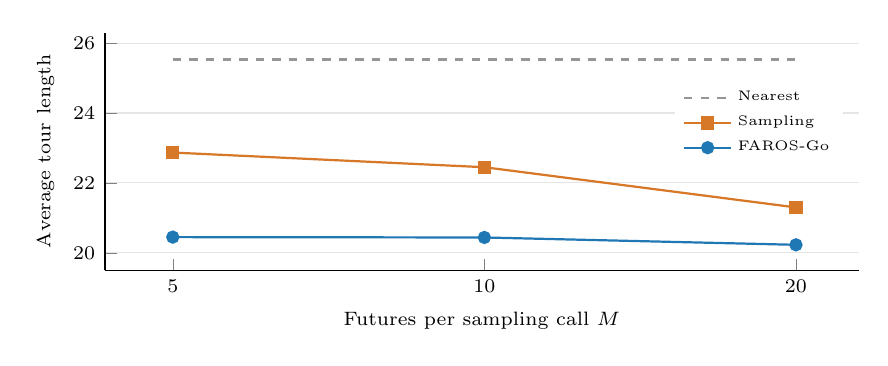
\begin{tikzpicture}
\begin{axis}[
  width=0.92\columnwidth, height=4.6cm,
  xmode=log, log basis x=2,
  xtick={5,10,20}, xticklabels={5,10,20},
  xmin=4.3, xmax=23,
  ymin=19.5, ymax=26.3,
  xlabel={Futures per sampling call $M$},
  ylabel={Average tour length},
  ymajorgrids, grid style={gray!20},
  axis lines*=left,
  tick label style={font=\scriptsize}, label style={font=\scriptsize},
  legend style={font=\tiny, draw=none, fill=white, at={(0.98,0.62)}, anchor=east},
  legend cell align=left
]
\addplot[cnear, dashed, thick] coordinates {(5,25.53) (10,25.53) (20,25.53)};
\addplot[cmsa, thick, mark=square*] coordinates {(5,22.87) (10,22.45) (20,21.30)};
\addplot[chyb, thick, mark=*] coordinates {(5,20.45) (10,20.44) (20,20.23)};
\legend{Nearest, Sampling, FAROS-Go}
\end{axis}
\end{tikzpicture}
\caption{Sampling depends strongly on the number of futures; FAROS-Go barely does, and with five futures it already beats sampling with twenty.}
\label{fig:ablation-m}
\end{figure}

\subsection{Simulation effort}
\label{sec:compute}

Table~\ref{tab:compute} counts sampling calls per seed over the four test days (Q5). Sampling calls the simulation at every fork, 801.9 times per seed, and simulates 57,008 futures. FAROS-Go makes 561.5 calls (30\% fewer) and simulates 35,582 futures (38\% fewer). FAROS-All meets 1,191.7 forks per seed and calls the simulation at 583.8 of them (27\% fewer calls than sampling); the waiting rule settles the other half without simulation. Our method is therefore both better and cheaper than the sampling method it builds on.

\begin{table}[t]
\centering
\footnotesize
\caption{Simulation effort per seed (four test days, $M=20$).}
\label{tab:compute}
\begin{tabular}{@{}lrr@{}}
\toprule
Policy & Sampling calls & Simulated futures \\
\midrule
Sampling & 801.9 & 57{,}008 \\
FAROS-Go & 561.5 & 35{,}582 \\
FAROS-All & 583.8 & not logged \\
Nearest, wait rule & 0 & 0 \\
\bottomrule
\end{tabular}
\end{table}

\subsection{Days without waves}
\label{sec:uniform}

To check whether the gains depend on the wave structure, we generated days with uniformly scattered customers and request times spread uniformly over the whole day. On these days we trained a learned scorer to predict the cost of completing the day after each option and compared its choices with the nearest customer on 718 test decisions from four days. After the learned choice, the average completion cost is 45.09; after the nearest choice it is 45.06; the best possible single choice, known from the simulations, gives 44.83. The learned scorer recovers none of the small available gain. Without waves there is little to anticipate, and the nearest rule is already close to the best single decision. This is a decision-level check and not a full-tour comparison of the five policies.

\subsection{A learned dispatcher on wave days}
\label{sec:learned}

We also trained small neural networks on simulation labels from days 0--11 of three seeds and selected them on days 12--15 (Q6). Table~\ref{tab:learned} reports their tour lengths on days 16--19 of those seeds. A learned decision on whether to wait at forks shortens the tour from 26.06 to 24.58 on average, with a large spread across seeds. A learned scorer that never waits is worse than nearest dispatching. Both remain far from the waiting rule and from our method. We report this result to show that the gain does not require learning, not as a competing method.

\begin{table}[t]
\centering
\footnotesize
\caption{Learned dispatchers on three seeds (test days 16--19). Not directly comparable with the ten-seed averages of Table~\ref{tab:main}.}
\label{tab:learned}
\begin{tabular}{@{}lrr@{}}
\toprule
Policy & Avg.\ tour & SD (seeds) \\
\midrule
Nearest & 26.06 & 0.70 \\
Learned wait decision at forks & 24.58 & 5.15 \\
Learned customer choice, never waits & 26.34 & 2.08 \\
\bottomrule
\end{tabular}
\end{table}

\subsection{Summary of claims}

Table~\ref{tab:claims} lists every claim of the paper with its evidence. A claim is \emph{supported} if its Holm-adjusted test is below $0.05$, a \emph{point estimate} if the average favors it without that support, \emph{observed} if it is a measured count without a test, and \emph{not supported} if the evidence goes the other way.

\begin{table}[!htbp]
\centering
\caption{Claims and evidence. S: supported; P: point estimate; O: observed; N: not supported.}
\label{tab:claims}
\scriptsize
\setlength{\tabcolsep}{2.5pt}
\renewcommand{\arraystretch}{1.1}
\begin{tabular}{@{}>{\raggedright\arraybackslash}p{0.36\columnwidth}>{\raggedright\arraybackslash}p{0.52\columnwidth}c@{}}
\toprule
Claim & Evidence & \\
\midrule
Fork decisions shorten tours & All four policies beat nearest on 40/40 days & S \\
FAROS beats sampling & Go 31/40 ($p=0.003$); All 34/40 ($p=5\times10^{-5}$) & S \\
Sampling adds value after the rule & Go 29/40 ($p=0.019$); All 34/40 ($p=5\times10^{-5}$) & S \\
Wait rule alone beats sampling & 26/40, $p=0.16$ & P \\
FAROS-All beats FAROS-Go & 20/16/4, $p=0.62$ & N \\
Sampling loses through timing noise & $M$ 5$\to$20: sampling $-1.57$, Go $-0.22$; Go at $M{=}5$ beats sampling at $M{=}20$ & O \\
FAROS needs less simulation & 562 / 584 vs.\ 802 calls per seed & O \\
Learning gains without waves & 45.09 learned vs.\ 45.06 nearest & N \\
Learned matches rule-based & 24.58 (3 seeds) vs.\ 20.00--20.89 & N \\
\bottomrule
\end{tabular}
\end{table}

\FloatBarrier

% =========================================================================
\section{Discussion}
\label{sec:discussion}
% =========================================================================

\paragraph{Decide timing first}
Sampling and our method use the same simulation, the same base heuristic, and the same futures. The only difference is the order of the decisions, and that difference alone shortens tours on most days and reduces simulation. Dispatching systems that already use sampling or rollout can adopt the change without a new solver: use known structure to decide when to wait, and spend simulation on where to go.

\paragraph{Where the gain comes from}
The experiment with different $M$ locates the weakness of sampling in noise. Its deficit shrinks as $M$ grows, while our method hardly changes. Two practical consequences follow. A small simulation budget suffices once timing is decided by a rule, which helps when decisions must be fast. And results of sampling methods should always be reported together with $M$, because a method that looks weak at small $M$ may only be noisy.

\paragraph{FAROS-Go or FAROS-All}
FAROS-All has the lower average and the larger margin over sampling, but the direct comparison does not separate the two. FAROS-Go varies less across seeds and simulates fewer futures per call. We would use FAROS-Go when computation is limited and FAROS-All when the waiting rule is believed to miss useful waits.

\paragraph{Structure before learning}
The learned dispatcher gains nothing without waves and little with them, while a one-line rule based on the wave windows captures most of the gain. In this setting the first task is to find the structure that makes anticipation valuable. Learning becomes relevant when that structure is not known in advance, for example when wave windows must be estimated from historical requests.

% =========================================================================
\section{Limitations}
\label{sec:limitations}
% =========================================================================

\paragraph{One synthetic generator and known windows}
All days come from one generator with four waves of fixed length and spacing. The dispatcher knows every potential customer and the wave windows, and the simulation draws futures from the true request-time distribution. In practice windows must be estimated, and a wrong window would affect both the waiting rule and the simulation. We have not tested wrong windows, other numbers or overlaps of waves, or real request data.

\paragraph{The waiting rule}
With the benchmark settings the threshold $\Delta$ never binds, so the rule reduces to waiting while the current wave is incomplete. Its behavior with longer windows, where the threshold would matter, is untested. An earlier implementation compared the threshold with the actual next request time; rerunning all rule-based policies with the version described in Section~\ref{sec:method} reproduced every test-day result exactly, so no reported number depends on that detail.

\paragraph{Scope of the comparison}
We study one vehicle without time windows or request rejection, and all simulations complete the day with the nearest dispatcher. Full reoptimization at each request, consensus-based scenario planning with a full routing solver, and offline--online value approximation were not run. The study isolates the effect of the decision order under a fixed simulation; it does not establish a new state of the art for dynamic routing.

\paragraph{Sample size}
The comparisons rest on 40 test days. The supported results are clear, but the waiting rule versus sampling and FAROS-Go versus FAROS-All would need more days to be resolved. The simulated-future count for FAROS-All was not logged.

\paragraph{Learned dispatchers}
The learned dispatchers are small networks evaluated on three seeds, and the check without waves is reported at the level of single decisions. Stronger learned policies may do better.

% =========================================================================
\section{Conclusion}
\label{sec:conclusion}
% =========================================================================

When requests arrive in overlapping waves, a vehicle repeatedly has to choose between a nearby leftover, a distant new wave, and waiting. Existing sampling methods make this choice by simulating every option, waiting included. We showed that deciding the waiting question first, with a rule based on the known wave windows, and simulating only the remaining choice, shortens tours on the same days (20.23 and 20.00 against 21.30), wins on 31 and 34 of 40 days, and needs about 30\% fewer simulation calls. The improvement is largest when few futures are sampled, which points to sampling noise in the timing decision as its source. Future work should test the approach with estimated windows, real request data, several vehicles, and stronger planning inside the simulation.

\section*{Declaration of competing interest}
% AUTHOR CHECK
The authors declare that they have no known competing financial interests or personal relationships that could have appeared to influence the work reported in this paper.

\section*{Data availability}
% AUTHOR CHECK: repository URL or archive DOI.
The stored instances, per-day results, and evaluation code will be made available upon publication.

\FloatBarrier
\bibliographystyle{elsarticle-harv}
\bibliography{faros_references}

\end{document}

%%%%%%%%%%%%%%%%%%%%%%%%%%%%%%%%%%%%%%%%%%%%%%%%%%%%%%%%%%%%%%%%%%%%%%%%%%%%
% REVIEWER BACKLOG (ignored by LaTeX). Most serious first.
%%%%%%%%%%%%%%%%%%%%%%%%%%%%%%%%%%%%%%%%%%%%%%%%%%%%%%%%%%%%%%%%%%%%%%%%%%%%
%  R1  Known windows / true sampler. The rule and the simulation both use the
%      exact wave windows and the true request-time distribution. Expected
%      review: "oracle information". Fix: rerun with shifted/scaled windows
%      (e.g. +-1, +-2 time units, width x0.75 / x1.25) used by rule + sampler.
%  R2  Weak comparison method. Sampling uses a nearest-dispatcher rollout and
%      4 candidates. Expected review: "strawman". Fix: add consensus scenario
%      planning or a rollout with a better base heuristic, and periodic
%      reoptimization of visible customers.
%  R3  One generator. Fix: vary waves {3,4,6}, overlap {1,3,5}, window {8,12,16}
%      (window 12+ also makes Delta bind -- addresses R6).
%  R4  40 test days. Extending test days is cheap (~45 s per seed for the
%      three rule-based policies). Fix: 20 test days per seed (200 days).
%  R5  Missing numbers: FAROS-All simulated futures (log futures_scored in
%      lazy_factory_stats); bootstrap CIs for FAROS-Go/FAROS-All vs wait rule and
%      FAROS-All vs FAROS-Go; wall-clock time per decision.
%  R6  Delta never binds; the rule is "wait while the wave is incomplete".
%      Stated in the text; covered by R3.
%  R7  Days-without-waves check is decision-level with a different learner.
%      Fix: run all five policies on full uniform days (sampler window
%      = [0, H]).
%  R8  Learned results: 3 seeds, SD 5.15. Keep secondary or drop.
%  R9  References: verify every DOI and author list, especially
%      zhang2023dvrpreview, ulmer2019adp, baty2024combinatorial,
%      saintguillain2017ssvrptw.
%  R10 SD column uses population SD of seed means (np.std); say so or switch
%      to ddof=1.
%  R11 Naming: code/logs still use hybrid_wait_msa_go (= FAROS-Go) and lazy_msa
%      (= FAROS-All). State this mapping in the code release README.
%      Check that "FAROS" does not clash with an existing OR/VRP method name.
